\begin{figure}[ht]
  \centering
  \begin{subfigure}[c]{0.48\textwidth}
    \centering
    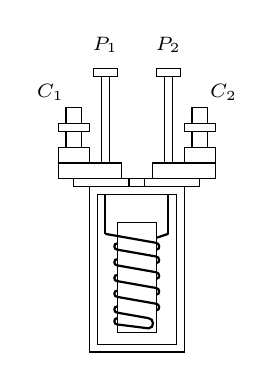
\begin{tikzpicture}
      % Inner core
      \draw (-0.25,0.15) rectangle (0.25,-1.25);
      % Window cut
      \draw (-0.5,0.5) rectangle (0.5,-1.4);
      % Outer wall
      \draw (-0.6,0.6) rectangle (0.6,-1.5);
      % Upper box rectangle and detail
      \draw (-0.8,0.7) rectangle (0.8,0.6);
      \draw (-0.1,0.7) rectangle (0.1,0.6);
      % Left and right terminal rectangles
      \draw (-1,0.9) rectangle (-0.2,0.7);
      \draw (0.2,0.9) rectangle (1,0.7);
      \draw (-1,1.1) rectangle (-0.6,0.9);
      \draw (0.6,1.1) rectangle (1,0.9);
      % C terminals
      \draw (-0.9,1.6) rectangle (-0.7,1.1);
      \draw[fill=white] (-1,1.4) rectangle (-0.6,1.3);
      \draw (0.7,1.6) rectangle (0.9,1.1);
      \draw[fill=white] (1,1.4) rectangle (0.6,1.3);
      \node at (-1.1,1.8) {\scriptsize{$C_1$}};
      \node at (1.1,1.8) {\scriptsize{$C_2$}};
      % P terminals
      \draw (-0.45,2) rectangle (-0.35,0.9);
      \draw (0.45,2) rectangle (0.35,0.9);
      \draw (-0.55,2.1) rectangle (-0.25,2);
      \draw (0.55,2.1) rectangle (0.25,2);
      \node at (-0.4,2.4) {\scriptsize{$P_1$}};
      \node at (0.4,2.4) {\scriptsize{$P_2$}};
      % the resistance
      \draw[thick] (-0.4,0.5) -- (-0.4,0);
      \draw[thick] (0.4,0.5) -- (0.4,0);
      \draw[thick] (0.4,0) -- (0.25,-0.05);
      \draw[thick] (-0.4,0) -- +(-10:0.65)
        to [out=0,in=0,looseness=1.5] +(0.65,-0.2);

      \foreach \y in {-0.2,-0.4,-0.6,-0.8}{
        \draw[thick] (-0.25,{\y+0.08}) to [out=180,in=180,looseness=1.5]
          (-0.25,\y) -- +(-10:0.5)
          to [out=0,in=0,looseness=1.5] +(0.5,-0.17);
      }
      \draw[thick] (-0.25,{-1+0.08}) to [out=180,in=180,looseness=1.5]
        (-0.25,-1) -- +(-10:0.4)
        to [out=0,in=0,looseness=1.5] +(0.4,-0.2) -- (-0.25,-1.15) 
        to [out=180,in=180,looseness=1.5] (-0.25,-1.07);
    \end{tikzpicture}
    \caption{Esquema representativo de la resistencia patrón.}
  \end{subfigure}
  \hfill
  \begin{subfigure}[c]{0.48\textwidth}
    \centering
    \begin{circuitikz}[european]
      \draw (-2,0) node[above]{$C_1$} to[short,o-*] (-1.25,0) coordinate (A)
        to[R=$R_\text{pat}$] (1.25,0) coordinate(B) to[short,*-o] (2,0) node[above]{$C_2$};

        \draw (A) -- ++(0,1.5) node[ocirc,label=above:$P_1$]{};
        \draw (B) -- ++(0,1.5) node[ocirc,label=above:$P_2$]{};
    \end{circuitikz}
    \vspace{1.5cm}
    \caption{Diagrama de circuito.}
  \end{subfigure}
  \caption{La conexión de Kelvin.}
  \label{fig_res_kelvin}
\end{figure}
